\documentclass[12pt]{article}
\usepackage[final]{graphicx}
\usepackage{amsfonts}
\usepackage{subfigure}

\topmargin-.5in
\textwidth6.6in
\textheight9in
\oddsidemargin0in

\def\ds{\displaystyle}
\def\d{\partial}

\begin{document}

%\centerline{\large \bf EPA}

%\vspace{.1truein}
%
%\def\thefootnote{\arabic{footnote}}
%\begin{center}
%  Neha Dilip Bora\footnote{Department, University},
%  Tuo Chen\footnote{Department, University},
%  Dana Victoria Cochran\footnote{Department, University},
%  Kelly Dougan\footnote{Department, University},
%  Gautam S  Sabnis\footnote{Department, University},
%  Chuanping Yu\footnote{Department, University}
%\end{center}
%
%%\vspace{.1truein}
%
%\begin{center}
%Faculty Mentors: Mentor 1\footnote{Company},
%Mentor 2\footnote{University}
%\end{center}
%
%
%\vspace{.3truein}
%\centerline{\bf Abstract}
%
%\begin{itemize}
%\item Summarize the results presented in the report, and the contributions
%of your research.
%
%\item Readers should not have to look at the rest of the paper in order to 
%understand the abstract.
%
%\item Keep it short and to the point.
%\end{itemize}
%
\section{Introduction}
%(It should be written as much as possible in non-technical terms, so that a
%lay reader can understand the context and the contribution of the paper.)
%
%Long term exposure to PM$_{2.5}$ is associated with human health complications (insert citation). Surface readings of PM$_{2.5}$ in the states on the West Coast of the United States have reported to be higher than allowed by the Clean Air Act. One possible reason for this is international transport of air pollution on PM$_{2.5}$. This project explores the relationship between the surface readings of PM$_{2.5}$ from coastal sites with the AOD measurements from the AVHRR in these regions. Once we found a correlation between these readings, we implemented a model to approximate PM$_{2.5}$ concentrations in the Pacific ocean, where surface readings are not possible.
%
%\begin{itemize}
%\item Describe the problem you are trying to solve, the approach
%you took, and summarize your contribution and results.
%
%\item (Review the history of this problem, and existing literature.) (add intro about AOD and PM2.5) Liu et al. used U.S. Environmental Protection Agency PM2.5 concentrations, Geostationary Operational Environmental Satellite aerosol/smoke product AOD, Meteorologic parameters, Spatial synoptic classification, land use parameters, and Spatial alignment of data to build a AOD model and non-AOD model for predicting PM2.5. It showed that by using AOD data, the prediction of PM2.5 concentrations would be more accurate. 
%
%
%\item Give an outline of the rest of the paper.
%\end{itemize}
%
\section{The Problem}
%
%The final goal of our project is to determine if there is any influence of international transport on the west coast of U.S., and if it does, how big the impact is. In order to do that, there are several problems we need to solve. 
%
%\subsection{Relationships between AVHRR AOD and surface PM2.5}
%Previous papers showed that there might be a strong correlation between the AOD and PM2.5. We may be able to use the AOD data to predict PM2.5. Since the sensors for detecting PM2.5 are only located on land, we cannot get the PM2.5 data on the ocean. We will use the PM 2.5 measurements on the west coast of the US along with the AOD data in this region to construct a model. We have used the surface measurements only on the coast to attempt to eliminate any contamination from traffic, civilization, etc. and to best model conditions on the ocean. 
%
%
%
%
%
%\begin{itemize}
%\item 
%
%\item State and justify all your assumptions. 
%
%\item Define notation. 
%
%\item Describe your data, how you collected them, their properties,
%and whether you did 
%anything to them (removed noise, filled in missing data, 
%applied normalizations).
%\end{itemize}

\section{The Approach}

\subsection{Identify U.S. PM2.5 sites within or adjacent to AVHRR grids}
As AVHRR satellites can only get the aerosol optical depth (AOD) from oceans and PM2.5 data are from lands, our strategy for identifying PM2.5 sites is to choose the ones that are as close to the coast as possible. Figure \ref{fig3.1} shows all the PM2.5 sites and Figure \ref{fig3.2}  shows the sites that we chose. We chose 13 PM2.5 sites closest to the west coast.

\begin{figure}[!h]
\centering
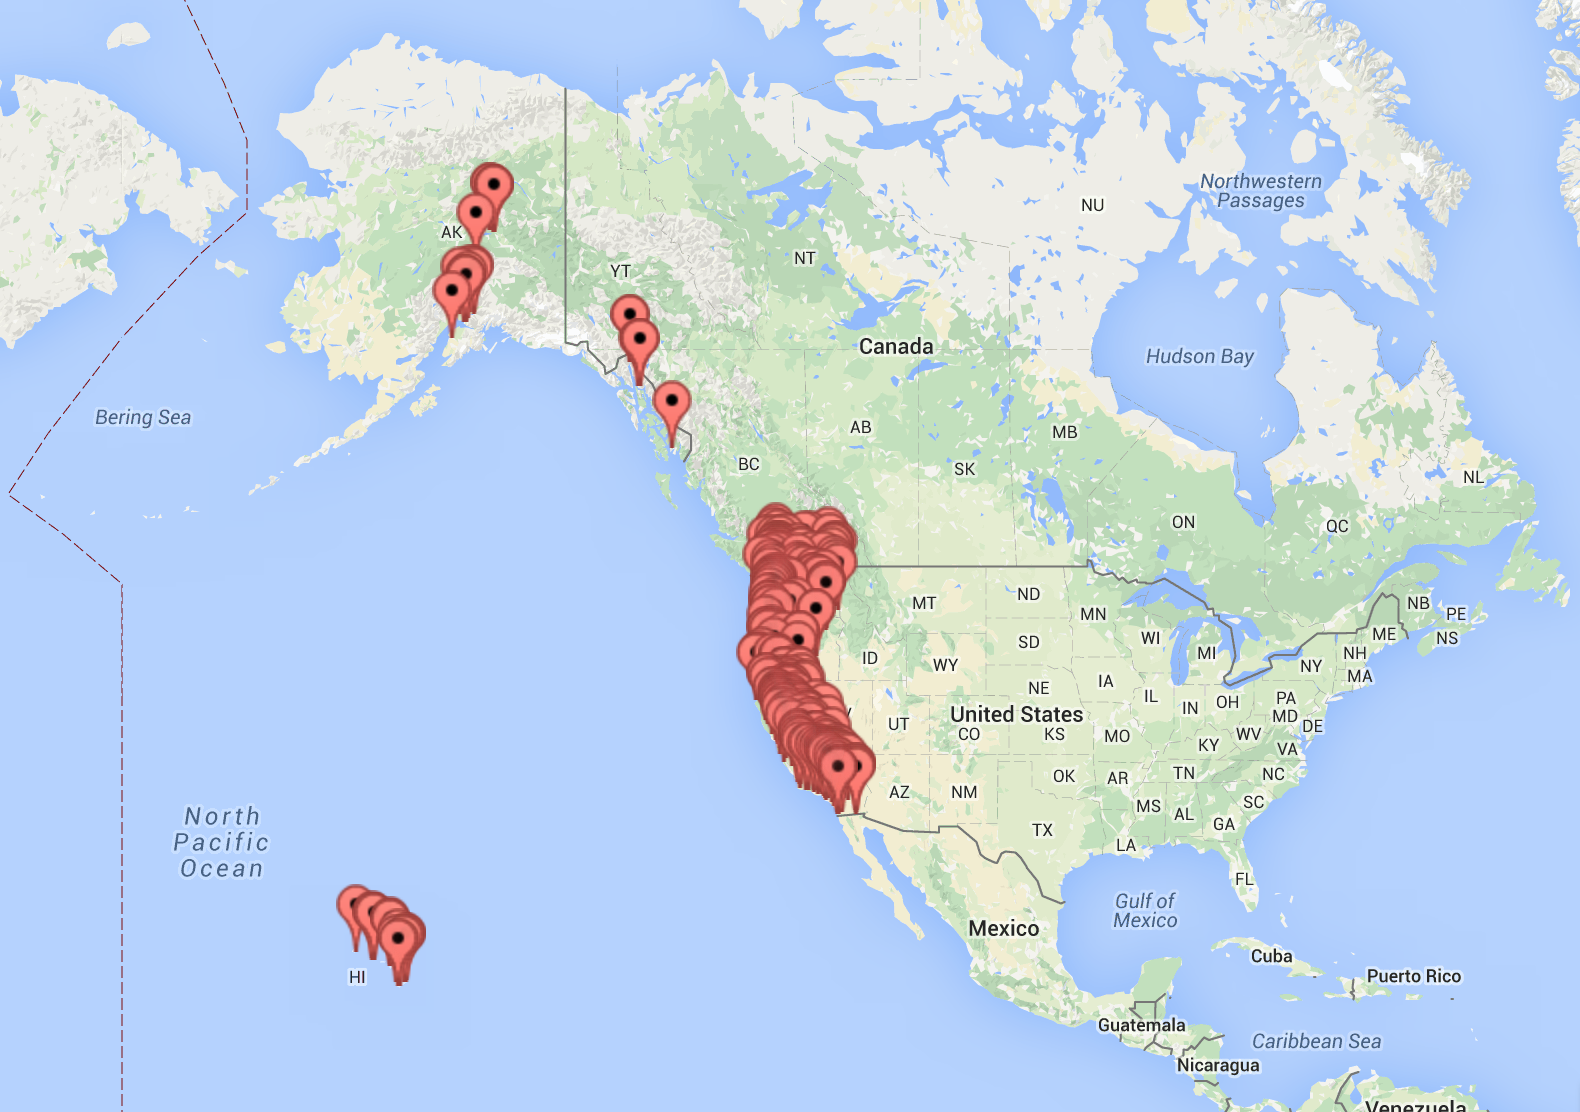
\includegraphics[width=0.8\linewidth]{AllPMSites.png}
\caption{All the PM2.5 sites}
\label{fig3.1}
\end{figure}

\begin{figure}[!h]
\centering
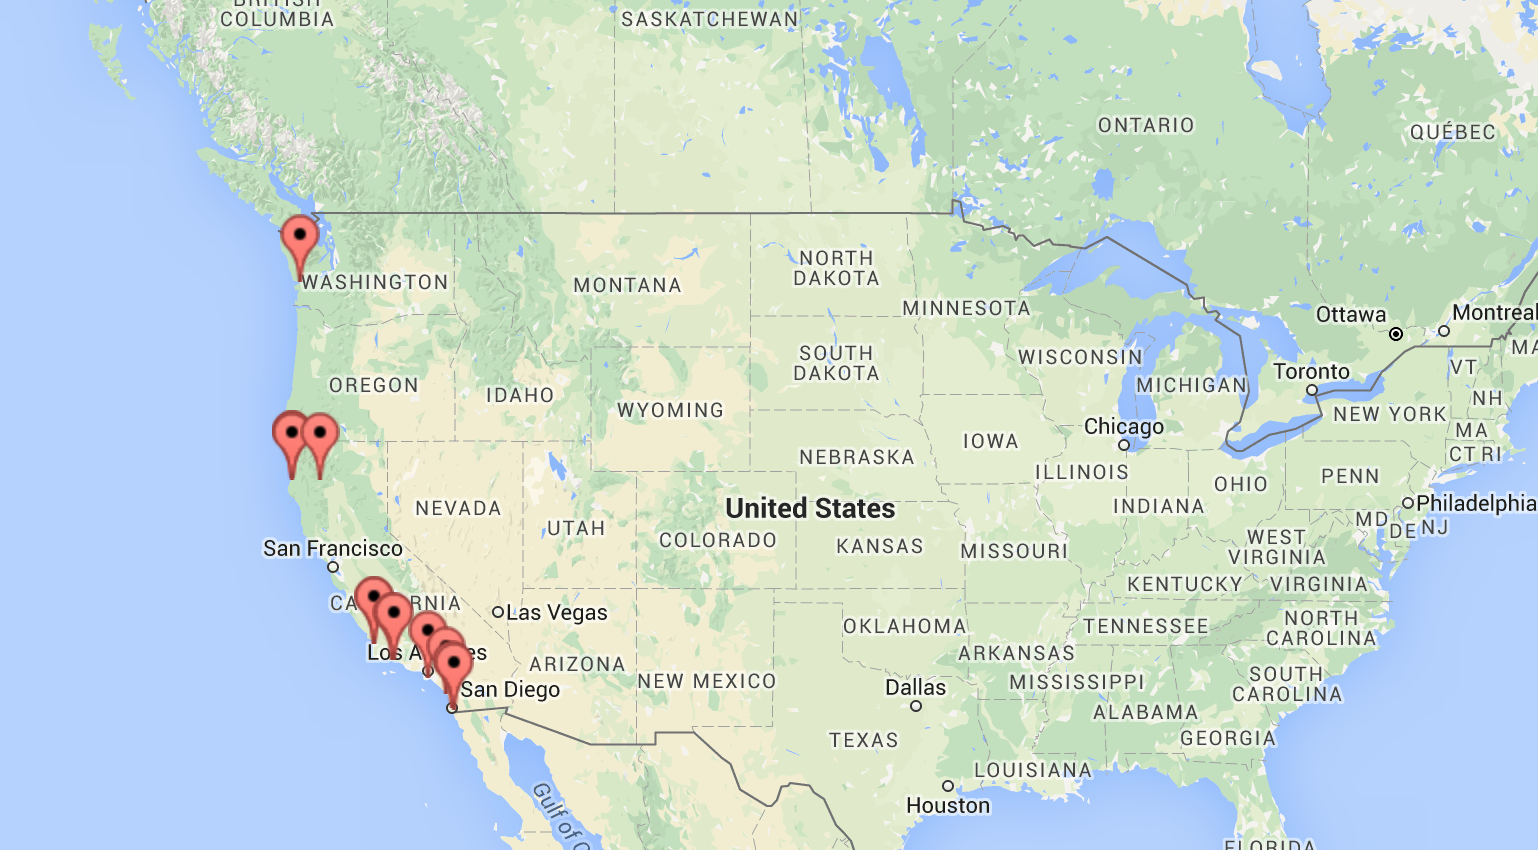
\includegraphics[width=0.8\linewidth]{PMSites.png}
\caption{PM2.5 sites chosen}
\label{fig3.2}
\end{figure}

%\begin{figure}
%\begin{minipage}[t]{0.5\linewidth}
%\centering
%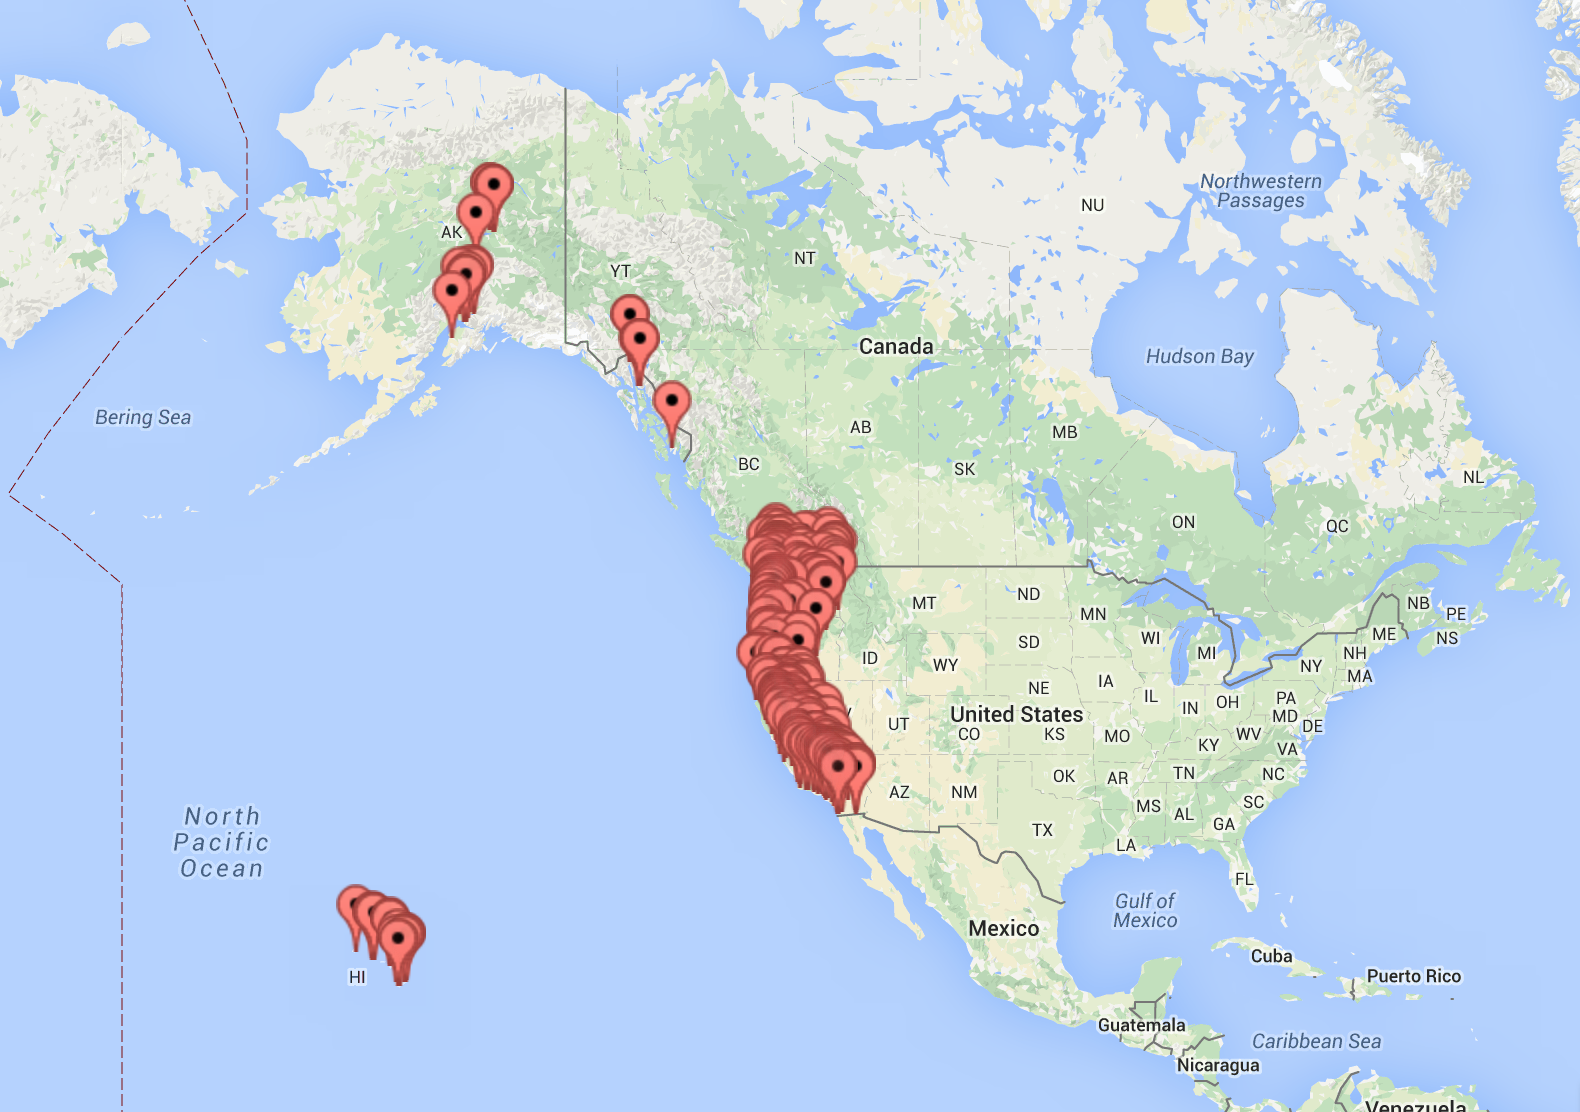
\includegraphics[height=2in]{AllPMSites.png}
%\caption{All the PM2.5 sites}
%\label{fig3.1}
%\end{minipage}
%\begin{minipage}[t]{0.5\linewidth}
%\centering
%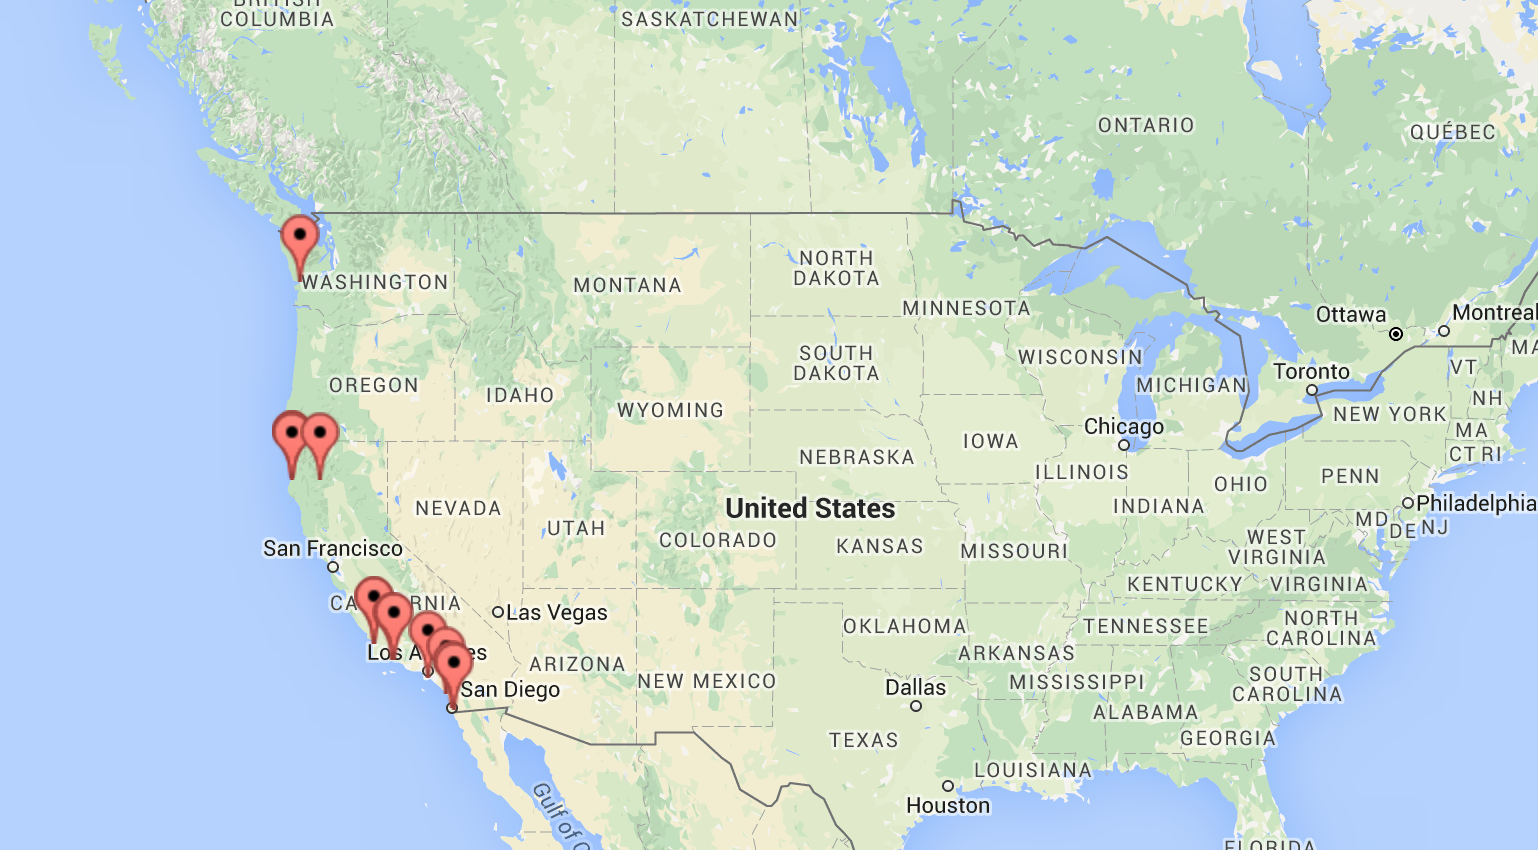
\includegraphics[height=2in]{PMSites.png}
%\caption{Chosen PM2.5 sites}
%\label{fig3.2}
%\end{minipage}
%\end{figure}

\subsection{Generate relationships between AVHRR AOD and surface PM2.5}
We noticed that there is huge differences between the sites we identified in the last step and the sites located on Hawaii. The sites we identified in the last step are all close to the west coast, while the sites located on Hawaii are far away from lands. So we decided to build models separately for both the sites we chose and the sites on Hawaii. 

\subsubsection{Clean the AVHRR AOD data}

No matter what PM2.5 sites we use, we need to find the closest AOD coordinates to the PM2.5 sites, and then to match the sites data for each day. This requires us to search all the observations in AOD dataset. The AOD data are very large and we cannot put all the data in hundreds of files into one matrix. Besides, AOD data have lots of missing data. So we need to clean the AOD data first. 

Since the data we want to use are the data located on the west coast and Hawaii, first we used the longitude and latitude of the west coast and Hawaii to eliminate data from other locations that we won\rq t use. Then, we dropped all the missing data and also changed the original format of the data into more readable one. Finally, our AOD data looks like Table \ref{table3.1}. 

\begin{table}[!h]
\centering
\begin{tabular}{|c|c|c|c|}
\hline 
Date & lat\_aot & long\_aot & aot\\
\hline
2000-01-25 & 30 & -126.6 & -0.0836133733391762 \\
\hline
$\cdots$ & $\cdots$ & $\cdots$ & $\cdots$\\
\hline
\end{tabular}
\caption{AOD data}
\label{table3.1}
\end{table}

\subsubsection{Match the AOD data with the PM2.5 data}
As we are trying to find the relationships between AOD and PM2.5, we need to keep all the date the same, and locations closest. After matching these two datasets, we got the following as in Table {table3.2}.

\begin{table}[!h]
\centering
\begin{tabular}{|c|c|c|c|c|c|c|}
\hline 
Date & lat\_pm & long\_pm & pm & lat\_aot & long\_aot & aot\\
\hline
2006-12-28 & 40.776944 & -124.1775 & 17.8 & 40.9 & -124.3 & 0.043815478682518\\
\hline
$\cdots$ & $\cdots$ & $\cdots$ & $\cdots$ & $\cdots$ & $\cdots$ & $\cdots$\\
\hline
\end{tabular}
\caption{AOD and PM2.5 match data}
\label{table3.2}
\end{table}

\subsubsection{relationships between AVHRR AOD and surface PM2.5 for sites closest to the west coast}

For sites closest to the west coast, we finally found 4 sites that have common date information. Figure \ref{fig3.3} is the plot regarding the AOD and PM2.5 by each site. 

\begin{figure}[!h]
\centering
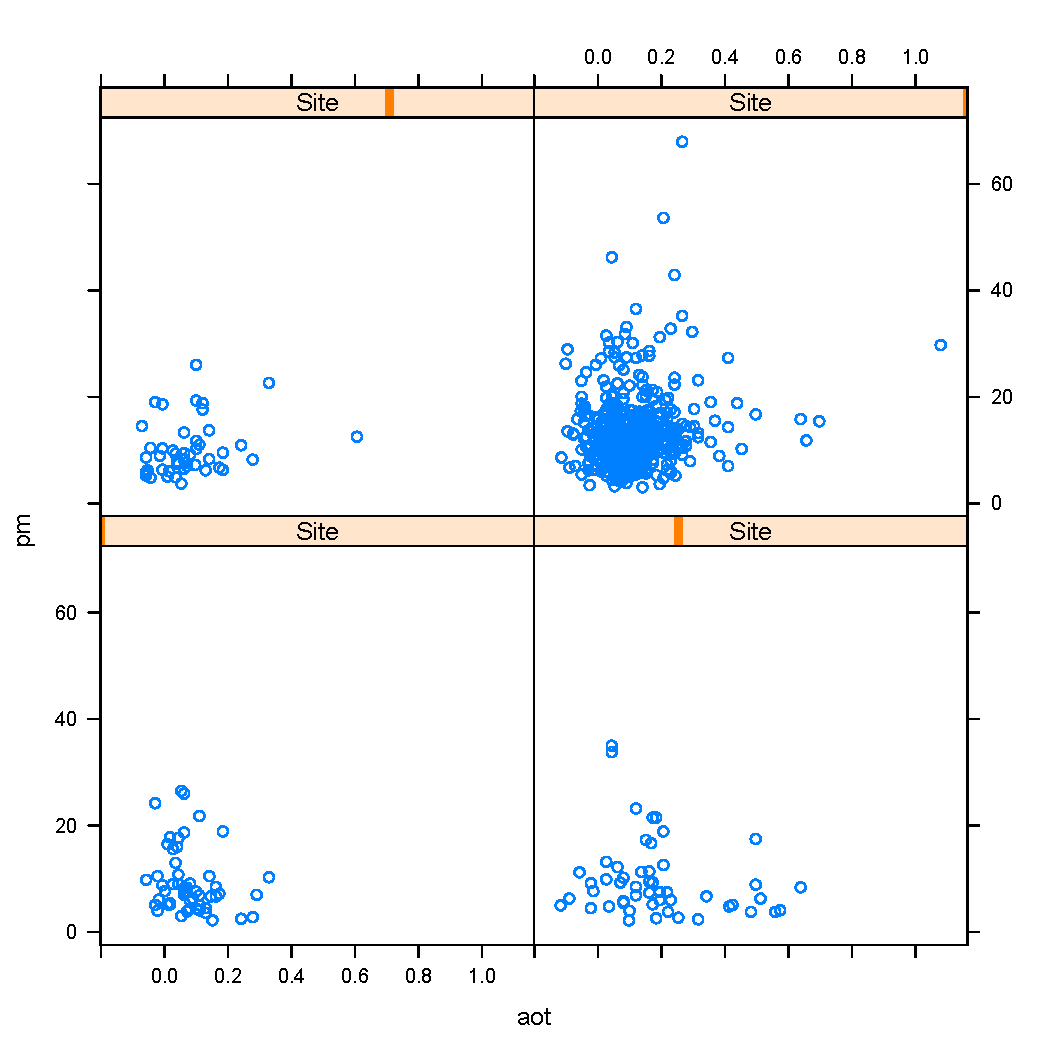
\includegraphics[width=\linewidth]{3.pdf}
\caption{PM vs. AOD for each site close to the west coast}
\label{fig3.3}
\end{figure}

We can see from the above plot that the relationships between AOD and PM2.5 are different for different sites. So we consider building different models for each site to find the relationships.

\subsubsection{relationships between AVHRR AOD and surface PM2.5 for Hawaii sites}

For Hawaii sites, we finally found 9 sites that have common date information. Figure \ref{fig3.4} is the plot regarding the AOD and PM2.5 by each site. 

\begin{figure}[!h]
\centering
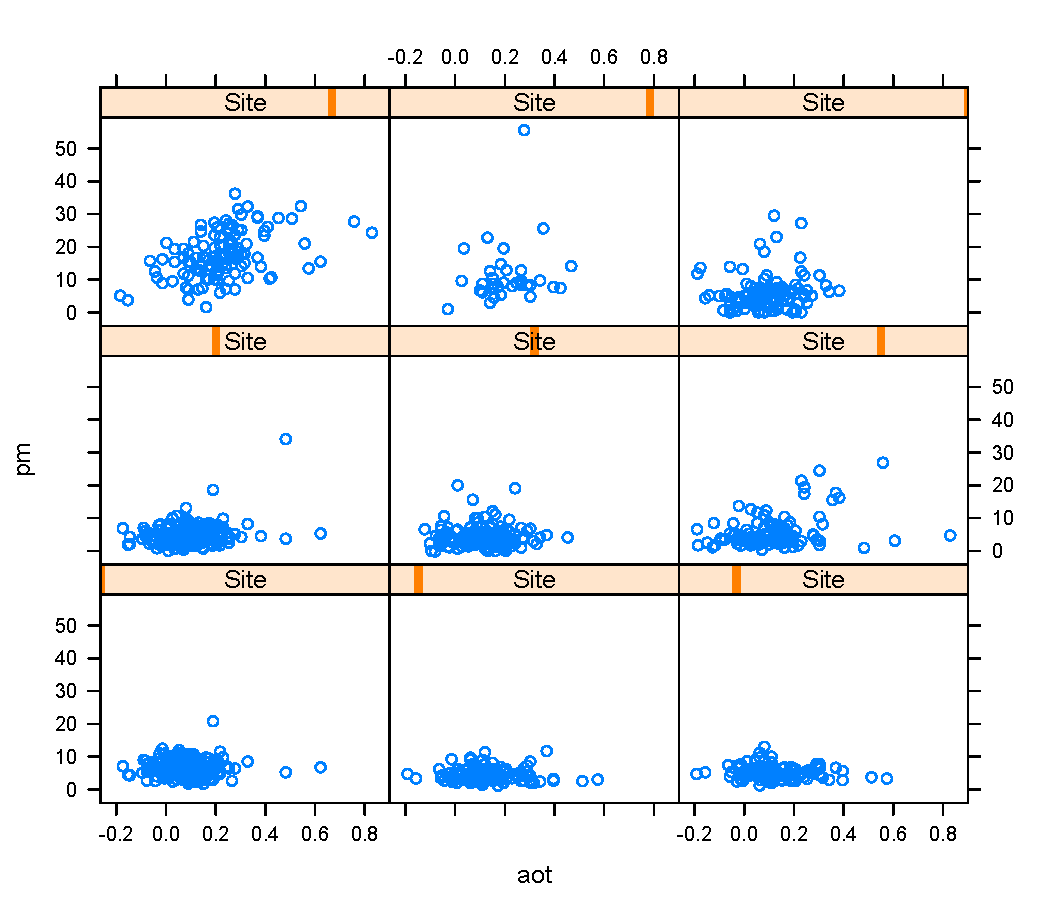
\includegraphics[width=\linewidth]{1.pdf}
\caption{PM vs. AOD for each Hawaii site}
\label{fig3.4}
\end{figure}

Similarly, we can see from the above plot that the relationships between AOD and PM2.5 are different for different sites. Like what we did for sites close to the west coast, we consider building different models for each site to find the relationships.




%\begin{itemize}
%\item Present and justify your approach for solving the problem. 
%\item Explain the advantages of your approach over existing ones.
%
%\item Tell a story.
%Don't just say: ``I did this, then I did this, and at last I did this''.
%\end{itemize}

%\section{Computational Experiments}
%Give enough details so that readers can duplicate your experiments.
%
%\begin{itemize}
%\item Describe the precise purpose of the experiments, and what they 
%are supposed to show.
%
%\item Describe and justify your test data, and any assumptions you made to 
%simplify the problem.
%
%\item Describe the software you used, and the 
%parameter values you selected.
%
%\item 
%For every figure, describe the meaning and units of the coordinate axes, 
%and what is being plotted.
%
%\item Describe the conclusions you can draw from your experiments
%\end{itemize}
%
%\section{Summary and Future Work}
%\begin{itemize}
%\item Briefly summarize your contributions, and their possible
%impact on the field (but don't just repeat the abstract or introduction).
%\item Identify the limitations of your approach.
%\item Suggest improvements for future work.
%\item Outline open problems.
%\end{itemize}



\end{document}

